\documentclass[a4paper]{article}
\usepackage[utf8x]{inputenc}
\usepackage[T1,T2A]{fontenc}
\usepackage[russian]{babel}
\usepackage{hyperref}
\usepackage{indentfirst} % включить отступ у первого абзаца
\usepackage{listings}
\lstset{inputpath=../listings}
\usepackage{color}
\usepackage{here} 
\usepackage{graphicx}
\graphicspath{{pics/}}

\usepackage{caption}
\renewcommand{\lstlistingname}{Листинг}

\usepackage{listings}
\lstdefinestyle{base_listing}{ %
extendedchars=\true,
basicstyle=\footnotesize,       % the size of the fonts that are used for the code
numbers=left,                   % where to put the line-numbers
numberstyle=\footnotesize,      % the size of the fonts that are used for the line-numbers
stepnumber=1,                   % the step between two line-numbers. If it is 1 each line will be numbered
numbersep=5pt,                  % how far the line-numbers are from the code
backgroundcolor=\color{white},  % choose the background color. You must add \usepackage{color}
showspaces=false,               % show spaces adding particular underscores
showstringspaces=false,         % underline spaces within strings
showtabs=false,                 % show tabs within strings adding particular underscores
frame=single,           % adds a frame around the code
tabsize=2,          % sets default tabsize to 2 spaces
captionpos=b,           % sets the caption-position to bottom
breaklines=true,        % sets automatic line breaking
breakatwhitespace=false,    % sets if automatic breaks should only happen at whitespace
escapeinside={\%*}{*)},          % if you want to add a comment within your code
postbreak=\raisebox{0ex}[0ex][0ex]{\ensuremath{\color{red}\hookrightarrow\space}},
keepspaces = true
}

\lstdefinestyle{crs_bash}{
  style    = {base_listing},
  language = {bash}
}

\lstdefinestyle{crs_cpp}{
  style    = {base_listing},
  language = {C++}
}

\usepackage[left=2.5cm, top=2cm, right=2cm, bottom=2cm, nohead]{geometry}

\begin{document}
\begin{titlepage} % начало титульной страницы

\begin{center} % включить выравнивание по центру

\large Санкт-Петербургский Политехнический Университет Петра Великого\\
\large Институт компьютерных наук и технологий \\
\large Кафедра компьютерных систем и программных технологий\\[6cm]
% название института, затем отступ 4,5см

\huge Операционные системы и среды\\[0.5cm]
\large Отчет по лабораторной работе №6\\[0.1cm]
\large Средства межпроцессного взаимодействия в ОС Windows\\[5cm]
\end{center}

\begin{flushright}
\begin{minipage}{0.5\textwidth}
\begin{flushright}
\textbf{Работу выполнил:}

Петров Владислав

{Группа:} 43501/4\\


\textbf{Преподаватель:} 

Душутина Елена Владимировна
\end{flushright}
\end{minipage} % конец врезки
\end{flushright} % конец выравнивания по левому краю

\vfill % заполнить всё доступное ниже пространство

\begin{center}

\large Санкт-Петербург\\
\large \the\year % вывести дату

\end{center} % закончить выравнивание по центру

\thispagestyle{empty} % не нумеровать страницу
\end{titlepage} % конец титульной страницы

\vfill % заполнить всё доступное ниже пространство


\section{Цель работы}
	Изучить средства межпроцессного взаимодействия в ОС Windows.
	
\section{Программа работы}
\begin{enumerate}
\item Неименованные каналы.\\
1.1. Создать клиент-серверное приложение, позволяющее набираемые символы в терминальном окне командной строки (сервер) отображать их в окно процесса-потомка (клиент).\\
1.2.Создать эхо-сервер, взаимодействующий с клиентом посредством pipe.
\item Именованные каналы.\\
2.1.Программа, обеспечивающая взаимодействие процессов посредством именованных каналов.Реализовать между одним клиентом и сервером обмен данными, вводимыми с консоли на стороне клиента и возвращаемыми сервером обратно до получения команды exit.\\
2.2. Программа, обеспечивающая взаимодействие процессов посредством именованных каналов – аналогичная программа с эхо-сервером, но с множеством клиентов и принудительной блокировкой обмена до завершения каждой операции. Реализовать между сервером и множеством клиентов обмен данными, вводимыми с консоли на стороне клиента и возвращаемыми сервером обратно до получения команды exit.\\
2.3. Модифицируем приложение из предыдущего примера (2.2) для сетевого обмена информацией.
\item Сокеты.\\
3.1. Программа локального обмена сокетами с использованием потокового протокола с установлением соединения (TCP в стеке TCP/IP).\\
3.2. Модифицировать программу для локального обмена с множеством клиентов и с доступом к общему ресурсу.\\
3.3. Сетевая передача данных с помощью сокетов.
\item  Провести эксперимент с множеством клиентов при сетевом обмене, представить результаты для виртуальной и реальной сетей;
\item  Проанализировать пример применения сокетов (сетевой обмен «мгновенными» сообщениями). Представить архитектуру приложения, алгоритмы сервера и клиента, схему и диаграмму их взаимодействия. Составить спецификацию функций (имя, назначение, параметры, файлы). Дополнить приложение, предоставив возможность обмениваться информацией клиентам в Linux и Windows. Исходный код в приложении. Настроить функционирование в лабораторной сети. Описать необходимые настройки.
\item  Привести примеры использования портов завершения. Привести пример приложения с большим количеством клиентов до 1000 (когда порты завершения оправданы), общее количество потоков не более 10.
\item  Оформить приложение с сокетами в виде службы.
\item  Реализовать обмен на основе UDP
\item  Сигналы в Windows\\
9.1. В качестве примера рассмотрим код из msdn. В нем происходит перехват сигналов CTRL+C, CTRL+BREAK. При этом обработчик смотрит, какой сигнал ему передан, и выводит его название. В качестве звуковой индикации работы приложение вызывает функцию Beep.\\
9.2. Предложить собственную реализацию обработчика сигнала.
\item Взаимодействие двух процессов через совместно используемую именованную память, при котором первый процесс записывает данные, а второй считывает их. Создать программу, в которой первый процесс генерирует случайное число и записывает его в буфер, доступный второму процессу, откуда он его и считывает с последующим выводом.
\item  Предложить собственную реализацию приложения, иллюстрирующую обмен информацией почтовыми слотами. Продемонстрировать возможность локального и удаленного доступа. Выполнить широковещательную передачу данных.
\end{enumerate}

\section{Ход работы}
Основная рабочая станция:\begin{lstlisting}[frame=rltb,numbers=none]
OS Name:                   Microsoft Windows 10 Pro
OS Version:                10.0.10586 N/A Build 10586
...
Wireless LAN adapter Wi-Fi 2:

   Connection-specific DNS Suffix  . :
   Link-local IPv6 Address . . . . . : fe80::58c4:2b5b:1f7:4fa7%6
   IPv4 Address. . . . . . . . . . . : 192.168.1.27
   Subnet Mask . . . . . . . . . . . : 255.255.255.0
   Default Gateway . . . . . . . . . : 192.168.1.1
	\end{lstlisting}
	
Дополнительная рабочая станция:\begin{lstlisting}[frame=rltb,numbers=none]
OS Name:                   Microsoft Windows 10 Pro
OS Version:                10.0.10586 N/A Build 10586
...
Ethernet adapter Ethernet:

   Connection-specific DNS Suffix  . :
   Link-local IPv6 Address . . . . . : fe80::a593:35fa:9f2:9f2c%4
   IPv4 Address. . . . . . . . . . . : 192.168.1.36
   Subnet Mask . . . . . . . . . . . : 255.255.255.0
   Default Gateway . . . . . . . . . : 192.168.1.1
	\end{lstlisting}
Стоит заметить, что дополнительная рабочая станция является виртуальной машиной с прямым доступом в локальную сеть. Использовался компилятор MinGW 4.9.2 x32.

\subsection{Неименованные каналы (Pipe)}
	Посредством pipe-канала можно передавать данные только между двумя процессами. В основе взаимодействия лежит так называемая файловая модель функционирования. Один из процессов создает канал, другой открывает его. После этого оба процесса могут передавать данные через канал в одну или обе стороны, используя для этого функции, предназначенные для работы с файлами, такие как \textbf{ReadFile} и \textbf{WriteFile}.
	
	Анонимные каналы (anonymous channels) Windows обеспечивают однонаправленное (полудуплексное) посимвольное межпроцессное взаимодействие. Каждый канал имеет два дескриптора: дескриптор чтения (read handle) и дескриптор записи (write handle).
	
	После создания канала необходимо передать клиентскому процессу его дескрипторы (или один из них), что обычно делается с помощью механизма наследования. Для наследования описателя нужно, чтобы процесс-потомок создавался функцией CreateProcess с флагом наследования TRUE.
	
	\textbf{Задание} Создать клиент-серверное приложение, позволяющее набираемые символы в терминальном окне командной строки (сервер) отображать их в окно процесса-потомка (клиент).
В программе-сервере master создается неименованный канал для связи с процессом-потомком, порождается сам процесс-потомок (программа-клиент) slave. На стороне сервера производится запись из консоли в канал. В slave открывается неименованный канал и осуществляется считывание из него в новое окно. Запись/чтение канала производится с помощью стандартных потоков \texttt{std\_in} и \texttt{std\_out}.

	Исходный код программы pipe\_master:
	\lstinputlisting[style=crs_cpp]{pipe_master.cpp}
	
	
	Исходный код программы pipe\_slave:
	\lstinputlisting[style=crs_cpp]{pipe_slave.cpp}
	
	При запуске "сервера" в командной строке выводится текст "Pipe Created!", затем сервером порождается процесс "slave" в новом окне, после чего любые символы, которые пишем в окне сервера, моментально появляются в окне клиента.
	\begin{figure}[h!]
		\center{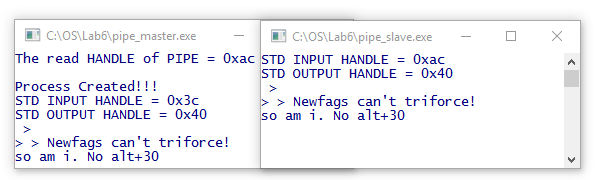
\includegraphics[scale=1]{task1}}
		\caption{Результат работы}
		\label{img:task1}
	\end{figure}
	
	\textbf{Задание} Создать эхо-сервер, взаимодействующий с клиентом посредством pipe.
	
	В программе используется передача дескрипторов через наследование. По причине того, что анонимный канал является полудуплексным, для организации эхо-сервера необходимо создавать 2 канала (для передачи от клиента-серверу и обратно). При этом ненужные дескрипторы каналов закрываются только на стороне сервера (т.к. клиент наследует 4 дескриптора, а явно мы передаем только 2 дескриптора).
	
	Дескрипторы каналов связываются со стандартным вводом и выводом клиентского процесса. Поэтому клиент выводит информацию в поток ошибок (что приведет к выводу в консоль процесса-клиента).
Клиент передает сообщение, например, вида: «message num 1». Сервер передает данное сообщение обратно. Процессы завершаются после передачи 10 сообщений.

	Исходный код программы сервера:
	\lstinputlisting[style=crs_cpp]{pipe_server.cpp}
	
	
	Исходный код программы клиента:
	\lstinputlisting[style=crs_cpp]{pipe_client.cpp}
	
	Результат выполнения программ:
	Сервер:
	\lstinputlisting[style=crs_cpp]{pipe_server.log}
	Клиент:
	\lstinputlisting[style=crs_cpp]{pipe_client.log}

	
\subsection{Именованные каналы}
	Именованные каналы являются дуплексными, ориентированы на обмен сообщениями и обеспечивают взаимодействие через сеть. Кроме того, один именованный канал может иметь несколько открытых дескрипторов. В сочетании с удобными, ориентированными на выполнение транзакций функциями эти возможности делают именованные каналы пригодными для создания клиент-серверных систем. Обмен данными может быть синхронным и асинхронным.
	
	Для создания именованного канала используется функция\\ \textbf{CreateNamedPipe}. При первом вызове функции CreateNamedPipe происходит создание самого именованного канала, а не просто его экземпляра. Закрытие последнего открытого дескриптора экземпляра именованного канала приводит к уничтожению этого экземпляра (обычно существует по одному дескриптору на каждый экземпляр). Уничтожение последнего экземпляра именованного канала приводит к уничтожению самого канала, в результате чего имя канала становится вновь доступным для повторного использования.
	
	После создания именованного канала сервер может ожидать подключения клиента, вызывая функцию \textbf{ConnectNamedPipe}.
	
	Для подключения клиента к именованному каналу применяется функция \textbf{CreateFile}.
	
	С помощью функции \textbf{WaitNamedPipe} процесс может выполнять ожидание момента, когда канал Pipe будет доступен для соединения.
	
	\textbf{Задание} Реализовать между одним клиентом и сервером обмен данными, вводимыми с консоли на стороне клиента и возвращаемыми сервером обратно до получения команды exit.

	Программа-сервер создает именованный канал для двунаправленного использования и ожидает подключения программы-клиента.
	
	Проверяем, корректно ли произошло подключение, затем входим в цикл получения команд от "клиента" с последующими эхо-ответами. При появлении команды exit со стороны клиента, сервер завершает работу, закрывает канал.
	
	Клиент на своей стороне открывает канал, пишет в него и читает эхо-ответ. При вводе exit программа завершается.
	
	Исходный код программы nppipe\_server:
	\lstinputlisting[style=crs_cpp]{npipe_server.cpp}
	
	Исходный код программы npipe\_client:
	\lstinputlisting[style=crs_cpp]{npipe_client.cpp}
	
	Результат выполнения программы приведен на рисунке \ref{img:task3}.
	\begin{figure}[h!]
		\center{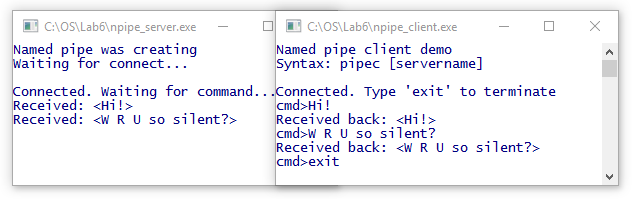
\includegraphics[scale=0.8]{task3}}
		\caption{Результат работы}
		\label{img:task3}
	\end{figure}
	
	Запускаем в одном окне сервер (на рис. слева). Он выводит сообщения о том, что канал создан и ожидает подключения клиента. Запускаем в другом окне клиента (справа). Затем на стороне сервера мы получаем уведомление о том, что создано новое подключение, теперь мы можем получать сообщения от клиента.
	
	Клиент после запуска выводит уведомления о том, что он подключился к серверу и ожидает ввода команд в строке cmd> . Вводимые в командной строке символы он пересылает серверу и сразу выводит возвращенный эхо-ответ от него. Для завершения сеанса обмена следует ввести зарезервированную команду exit на стороне клиента, после ее доставки серверу, он завершает работу.
	
	Сервер работает с одним клиентом, поэтому ему не нужно вызывать функции отсоединения клиента (по завершению сервера, клиент тоже завершается).\\
	
	\textbf{Задание} Реализовать между сервером и множеством клиентов обмен данными, вводимыми с консоли на стороне клиента и возвращаемыми сервером обратно до получения команды exit.
	
	Сервер, как и ранее, создает все необходимые ресурсы и переходит в состояние ожидания соединений. Именованный канал создается для чтения и записи. Передача происходит сообщениями, функции передачи и приема блокируются до их окончания.
	
	Клиент после соединения с сервером начинает чтение сообщений с консоли, пока не встретит слово «exit». По данному слову и клиент и сервер завершают свою работу.
	
	Обратить внимание на использование функции WaitNamedPipe, а также на возможность использования количества экземпляров каналов, равного количеству потенциальных клиентов.
	
	Исходный код программы npipe\_server\_bi:
	\lstinputlisting[style=crs_cpp]{npipe_server_bi.cpp}
	
	
	Исходный код программы npipe\_client\_bi:
	\lstinputlisting[style=crs_cpp]{npipe_client_bi.cpp}
	
	Результат выполнения программы приведен на рисунке \ref{img:task4}.
	\begin{figure}[h!]
		\center{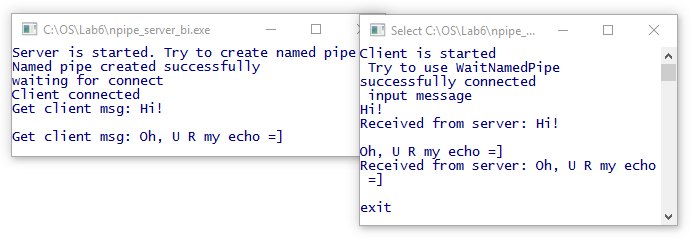
\includegraphics[scale=0.8]{task4}}
		\caption{Результат работы}
		\label{img:task4}
	\end{figure}
	
	Для подключения нескольких клиентов сервер был изменен:
	\lstinputlisting[style=crs_cpp]{npipe_server_bi_multi.cpp}
	
	Результат выполнения программы приведен на рисунке \ref{img:task4_2}.
	\begin{figure}[h!]
		\center{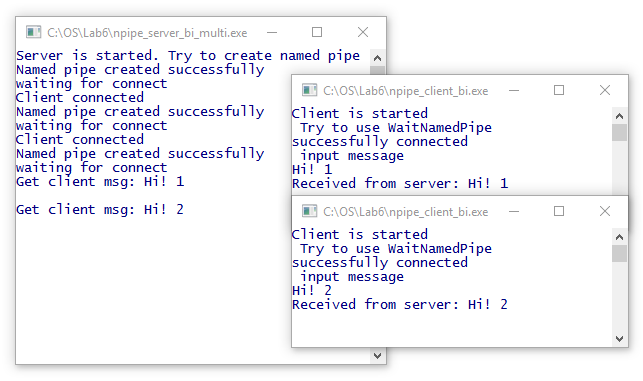
\includegraphics[scale=0.8]{task4_2}}
		\caption{Результат работы}
		\label{img:task4_2}
	\end{figure}
	
	Именованные каналы позволяют осуществлять обмен между процессами, выполняющимися на разных компьютерах в сети. Для этого необходимо выполнить определенный ряд условий и настроек. Но сетевые именованные каналы не являются промышленным стандартом и используются в этом качестве скорее как исключение. В ОС семейства Windows это возможно, в отличие, например, от Unix-подобных систем, где обмен данными осуществляется через ядро.
	
	Для совместной работы компьютеры нужно подсоединить к одной домашней группе. Так же необходимо установить поле DACL (Discretionary Access Control List) защиты объекта в NULL (разрешение всем пользователям и группам доступа к объекту). Параметры защиты именованного канала задаются с помощью структуры SECURITYATTRIBUTES, которая указывается последним параметром в функции CreateNamedPipe.
	
	Server для работы по сети:
	\lstinputlisting[style=crs_cpp]{npipe_server_bi_multi_net.cpp}
	
	Client для работы по сети:
	\lstinputlisting[style=crs_cpp]{npipe_client_bi_net.cpp}
	
	Программы были протестированы в локальной сети. Программы npipe\_server\_bi\_multi\_net и npipe\_client\_bi\_net запускались на разных машинах с ОС Windows 10. Компьютеры были объединены в общую домашнюю группу.
	
	Результат работы npipe\_server\_bi\_multi\_net на основной машине приведен на рисунке \ref{img:task5m}.
	\begin{figure}[h!]
		\center{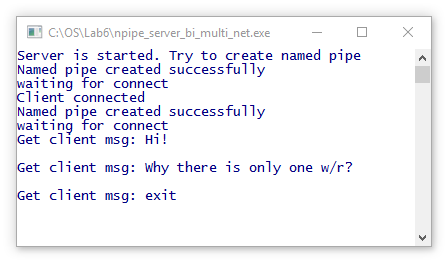
\includegraphics[scale=0.8]{task5m}}
		\caption{Результат работы npipe\_server\_bi\_multi\_net}
		\label{img:task5m}
	\end{figure}
	
	Результат работы npipe\_client\_bi\_net на дополнительной машине приведен на рисунке \ref{img:task5s}.
	\begin{figure}[h!]
		\center{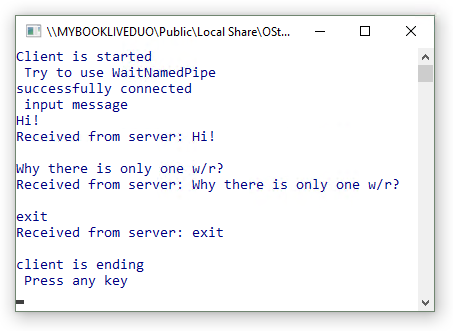
\includegraphics[scale=0.8]{task5s}}
		\caption{Результат работы npipe\_client\_bi\_net}
		\label{img:task5s}
	\end{figure}		
	
	Из-за сложности получения в программе собственных сетевых адресов для подтверждения общения по сети, было решено отловить трафик утилитой WireShark. Трафик отлавливался на основной машине (сторона сервера)
	
		Инициализация общения представлена на рисунке \ref{img:wireinit}.
	\begin{figure}[h!]
		\center{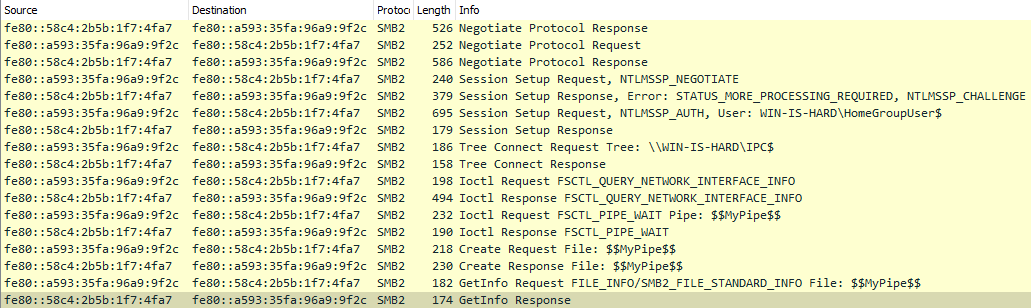
\includegraphics[scale=0.8]{wire_init}}
		\caption{Инициализация общения сервера и клиента}
		\label{img:wireinit}
	\end{figure}
	
	Пример записи и последующего чтения представлен на рисунке \ref{img:wiremsg}.
	\begin{figure}[h!]
		\center{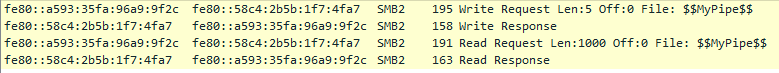
\includegraphics[scale=0.8]{wire_msg}}
		\caption{Один цикл обмена данными}
		\label{img:wiremsg}
	\end{figure}
	
	Этап завершения общения представлен на рисунке \ref{img:wireexit}.
	\begin{figure}[h!]
		\center{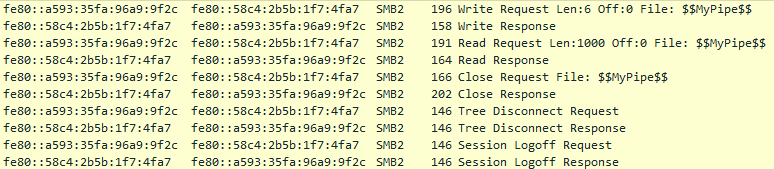
\includegraphics[scale=0.8]{wire_exit}}
		\caption{Инициализация общения сервера и клиента}
		\label{img:wireexit}
	\end{figure}
	
	Из записи трафика видно, что общение происходит между двумя машинами, а нагрузка на сеть достаточно велика.
\subsection{Сокеты}
	Возможность взаимодействия с другими системами обеспечивается в Windows поддержкой сокетов (sockets) Windows Sockets — совместимого и почти точного аналога сокетов Berkeley Sockets, де-факто играющих роль промышленного стандарта.
	
	Winsock API поддерживается библиотекой DLL (WS232.DLL), для получения доступа к которой следует подключить к программе библиотеку WS232.LIB. Эту DLL следует инициализировать с помощью нестандартной, специфической для Winsock функции WSAStartup, которая должна быть первой из функций Winsock, вызываемых программой. Когда необходимость в использовании функциональных возможностей Winsock отпадает, следует вызывать функцию WSACleanup. В QtCreator подключение происходит с помощью добавления в файл проекта (.pro) строчки "LIBS += -lws2\_32".
	
	После инициализации библиотеки сокетов можно использовать стандартные функции работы с сокетами.
	
	Взаимодействие в сети осуществляется между клиентом и сервером. Клиент посылает серверу некоторый запрос. Сервер обрабатывает запрос и шлет ответ. Сам по себе сокет – это оконечная точка соединения, которая идентифицируется 4 значениями: IP адрес отправителя, порт отправителя, IP адрес получателя, порт получателя. Порт – идентификатор процесса в ОС с точки зрения сетевого взаимодействия. Порт напрямую связан с протоколом. Например, в ОС могут быть два процесса с одинаковым номером порта, но использующие при этом разные протоколы.
	
	Программа локального обмена сокетами с использованием потокового протокола с установлением соединения (TCP в стеке TCP/IP). Для потоковых протоколов (к которым относится протокол TCP в стеке TCP/IP) необходимо применять средства, позволяющие определить границы сообщений в передаваемых данных, так как данный вид протоколов имеет дело с доставкой только потока байт (при этом гарантируется порядок доставки).
	
	Исходный код программы tcp\_server:
	\lstinputlisting[style=crs_cpp]{tcp_server.cpp}

	Основная функция программы tcp\_client:
	\begin{lstlisting}[style=crs_cpp]
	int main(void) { //используется для инициализации библиотеки сокетов
    WSADATA WSStartData; //Инициализация WinSock и проверка его запуска
    if (WSAStartup(MAKEWORD(2, 0), &WSStartData) != 0) {
        printf("WSAStartup failed with error: %ld\n", GetLastError());
        return 100;
    }
    int er_code=0; // инициализация клиентского сокета
    printf("Client is started.\nTry to create socket\n");
    int client_socket = socket( AF_INET, SOCK_STREAM, 0 );
    printf("socket created successfully\n");
    struct sockaddr_in sin;
    sin.sin_addr.s_addr=inet_addr("127.0.0.1");
    sin.sin_port=htons(7500);
    sin.sin_family=AF_INET; // установливаем TCP-соединение
    printf("try to connect to server\n");
    if(connect(client_socket, (struct sockaddr *) &sin,sizeof(sin))!=0) {
        printf("connect failed with error: %d\n", er_code);
        return SOCKET_ERROR;
    }
    printf("Client connected sucessfully\nEnter msg to send\n---------------------\n");
    char buf[SIZE_OF_BUF]; //буфер для приема и передачи сообщений
    while(1) {
        fgets(buf,SIZE_OF_BUF,stdin);
        printf("client sended msg: %s",buf);
        sendLine(client_socket,buf);
        recvLine(client_socket,buf,SIZE_OF_BUF);
        printf("get msg from serv: \"%s\"\n**********************\n",buf);
    } // заканчиваем работу с сокетом клиента
    closesocket(client_socket);
    return 0;
}	\end{lstlisting}
	
	Результат выполнения программы приведен на рисунке \ref{img:task6}.
	\begin{figure}[h!]
		\center{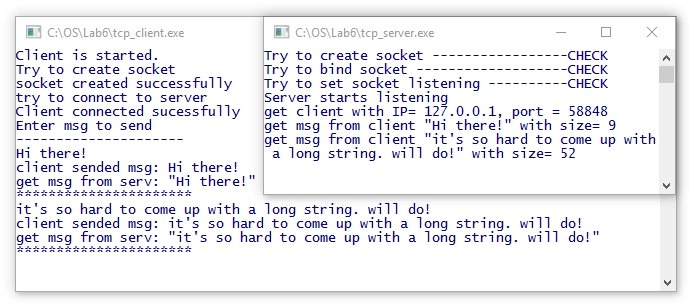
\includegraphics[scale=0.8]{task6}}
		\caption{Результат работы}
		\label{img:task6}
	\end{figure}
	
	Для поддержки подключения нескольких клиентов код сервера был немного изменен:
	\begin{lstlisting}[style=crs_cpp]
DWORD WINAPI threadHandler(LPVOID param){
	SOCKET client_socket = (SOCKET)param;
	if (client_socket == INVALID_SOCKET) {
		printf("error with accept socket. GetLasterror= %d\n", GetLastError());
		return 1003;
	}
	char buf[SIZE_OF_BUF]; //буфер приема и передачи сообщения 
	int readbytes; //число прочитанных байт 
	while (1) {
		if ((readbytes = recvLine(client_socket, buf, SIZE_OF_BUF)) == 0) {
			printf("Connection refused\n");
			break;
		}
		else if (readbytes == -1) {
			printf("buf is small\n");
			return 2000;
		}
		printf("get msg from client \"%s\" with size= %d\n", buf, readbytes);
		sendLine(client_socket, buf); //sendn(client_socket,buf,readbytes,0); //шлем сообщение обратно клиенту
		if (strncmp(buf, "exit", 4) == 0) break;
	}
	closesocket(client_socket);
	return 0;
}
//............
// main:
	while (SOCKET client_socket = accept(server_socket, (struct sockaddr*)&from, &fromlen)){
		HANDLE t;
		t = CreateThread(NULL, 0, threadHandler, (LPVOID)client_socket, 0, NULL);
	}
	closesocket(server_socket);
	\end{lstlisting}
	
	С помощью сокетов часто реализовывают сетевые приложения. Для этого необходимо внести незначительные изменения в код сервера и клиента: слушающий сокет сервера необходимо привязывать к адресу \texttt{INADDR\_ANY}, чтобы он мог принимать соединения с любых адресов; клиенту необходимо указать IP адрес компьютера, на котором запущен сервер.
	
	Результат выполнения сервера и двух клиентов рис. \ref{img:task6_2}. По этому рисунку видно, что общение происходило между разными компьютерами в сети.
	\begin{figure}[h!]
		\center{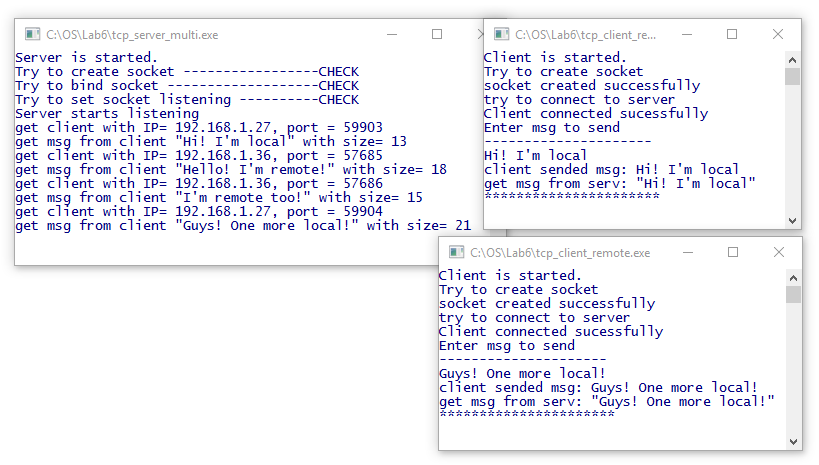
\includegraphics[scale=0.8]{task6_2}}
		\caption{Основная машина}
		\label{img:task6_2}
	\end{figure}	
	
	Результат выполнения двух удалённых клиентов \ref{img:task6_3}.
	\begin{figure}[h!]
		\center{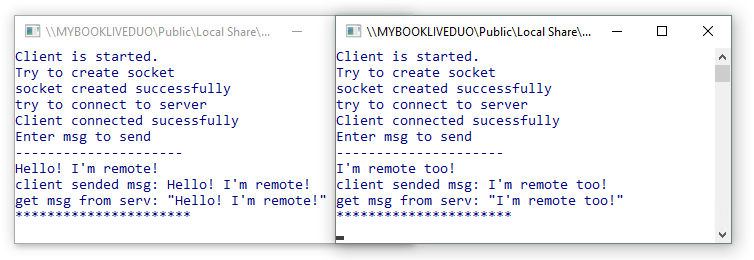
\includegraphics[scale=0.8]{task6_3}}
		\caption{Дополнительная (удалённая) машина}
		\label{img:task6_3}
	\end{figure}
	
Так мы видим, что с одним сервером могут работать сразу несколько клиентов, причём доступ открыт и из сети. Открытие доступа требует дополнительных прав при запуске программы, но получив права, сервер успешно запускается. Обеспечение доступа всех клиентов к общему ресурсу с помощью мьютекса является самым простым и надёжным решением, однако наименее эффективным.
	
\subsection{Порты завершения}
Порт завершения представляет собой специальный механизм в составе ОС, с помощью которого приложение использует объединение (пул) нескольких потоков, предназначенных единственно для цели обработки асинхронных операций ввода/вывода с перекрытием.
Для функционирования этой модели необходимо создание специального программного объекта ядра системы, который и был назван "порт завершения". Это осуществляется с помощью функции CreateIoCompletionPort(), которая асссоциирует этот объект с одним или несколькими файловыми (сокетными) дескрипторами и который будет управлять перекрывающимися I/O операциями, используя определенное количество потоков для обслуживания завершенных запросов. 

Опишем основной каркас прикладной программы-приложения, использующей для ввода/вывода модель порта завершения.  Это простой ECHO-сервер, получающий информацию от клиента и ее же обратно отправляющего. Предлагается следующие шаги:
\begin{enumerate}
\item Создать порт завершения. Четвертый параметр функции оставлен как 0 - только одному рабочему потоку на процессоре будут позволено выполняться в данное время на порте завершения.  
\item Создать рабочие потоки для обслуживания завершенных I/O-запросов на порте завершения. Когда вызывается функция создания потока CreateThread(), необходимо  указать ту функцию, которая будет исполняться в рабочем потоке. 
\item Сформировать слушающий сокет, чтобы принимать входные подключений на порту 7500.
\item Принять поступившие подключения функцией accept(). 
\item Создать структуру данных, чтобы представить "per-handle data" и сохранить дескриптор присоединенного сокета в структуре. 
\item Связать новый дескриптор сокета, возвращенный из accept(), с портом завершения,  вызывая CreateIoCompletionPort(). Передать структуру с "per-handle data" в функцию CreateIoCompletionPort() через параметр ключа завершения. 
\item Начать выполнять операции I/O на принятом подключении. По существу, мы будем выдавать один или более асинхронных вызовов WSARec() или WSASend() на новом сокете, используя  механизм ввода/вывода с перекрытием. Вызовы этих функций будут исполняться асинхронно и с перекрытием (т.е. одновременно). Когда эти функции завершатся (с тем или иным результатом), рабочий поток обслужит исполненные запросы и будет ждать следующие вызовы.	
\end{enumerate}

Исходный код программы tcp\_sever\_complition:
	\lstinputlisting[style=crs_cpp]{tcp_server_complition.cpp}
	
	Проверим работоспособности сервера в пределах локальной машины и пары ранее рассмотренных tcp клиентов клиентов, рисунок \ref{img:tcp_c_local_test}.
	\begin{figure}[h!]
		\center{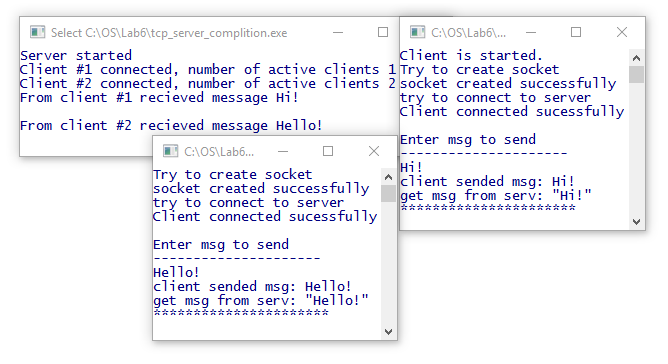
\includegraphics[scale=0.8]{tcp_c_local_test}}
		\caption{Локальная проверка}
		\label{img:tcp_c_local_test}
	\end{figure}
	
	Теперь запустим сервер в нагруженной ситуации. Для этого перепишем клиент, изменив адрес на адрес дополнительной рабочей станции, а ручной ввод текста заменим на вывод заданной строки через раз в 20 секунд. Напишем bat скрипт для запуска 1000 клиентов:
	\lstinputlisting[style=crs_cpp]{stress.bat}
	
	На дополнительной машине запустим сервер, а скрип на основной. Будем наблюдать за нагрузкой на дополнительной машине в установившийся период:
	\begin{figure}[h!]
		\center{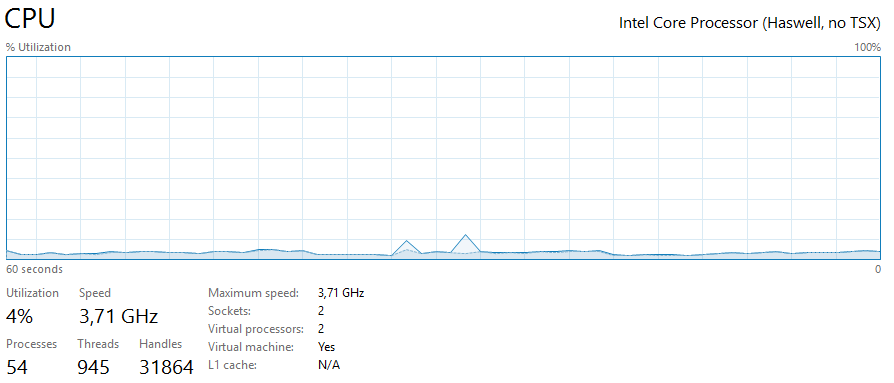
\includegraphics[scale=0.5]{stress_completion}}
		\caption{Нагрузка при использование завершающих портов}
		\label{img:stress_completion}
	\end{figure}
	
	Для осознания эффективности проведём такой же эксперимент но с обычным, многопоточным, tcp сервером:
	\begin{figure}[h!]
		\center{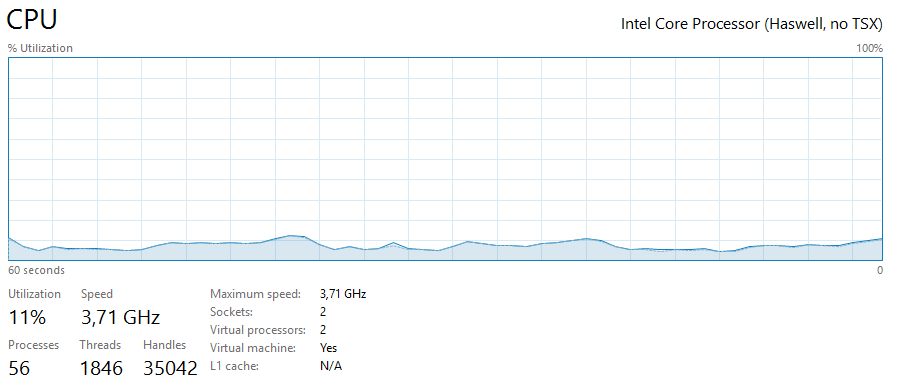
\includegraphics[scale=0.5]{stress_threads}}
		\caption{Нагрузка без использования завершающих портов}
		\label{img:stress_threads}
	\end{figure}
	
	При сравнение заметна разница в количестве потоков. А нагрузка на процессор выросла больше чем в два раза, это при том, что часть ресурсов использует и сама система. Таким образом порты завершения являются эффективным решением для многоклиентских приложений.
\subsection{Сигналы в Windows}
	Данное средство IPC в Windows не поддерживается. Однако, например, консольному приложению можно посылать сигналы CTRL+C и CTRL+BREAK. Система может посылать приложению сигналы: \texttt{CTRL\_CLOSE\_EVENT,\\ CTRL\_LOGOFF\_EVENT и CTRL\_SHUTDOWN\_EVENT}, когда пользователь закрывает консоль, выходит из системы, или когда система завершается. По получению данных сигналов процесс может произвести корректное завершение.
	
	С помощью функции SetConsoleCtrlHandler можно установить обработчик на данные сигналы, но отправить сигнал другому приложению мы не можем. 
	
	Зарегистрированный обработчик должен проверять тип сигнала на возможность его обработки. Обработчики сигналов объединены в список. Когда приходит сигнал, вызывается последний зарегистрированный обработчик (при этом запускается отдельный поток). Если этот обработчик возвращает FALSE (он не обрабатывает этот сигнал), то вызывается следующий. Если все обработчики вернули FALSE, вызовется обработчик по-умолчанию, который по-умолчанию завершает процесс.
	
	В качестве примера рассмотрим код из msdn. В нем происходит перехват сигналов CTRL+C, CTRL+BREAK. При этом обработчик смотрит, какой сигнал ему передан, и выводит его название. В качестве звуковой индикации работы приложение вызывает функцию Beep. Данная функция воспроизводит звуковой сигнал через динамик консоли с разной частотой и длительностью, задаваемыми ей через параметры.
	
	В функции main регистрируется обработчик сигналов, затем главный поток работает в бесконечном цикле.
	
	Искодный код:
	\lstinputlisting[style=crs_cpp]{signal.cpp}
	
	Результат выполнения программы приведен на рисунке \ref{img:task7}.
	\begin{figure}[h!]
		\center{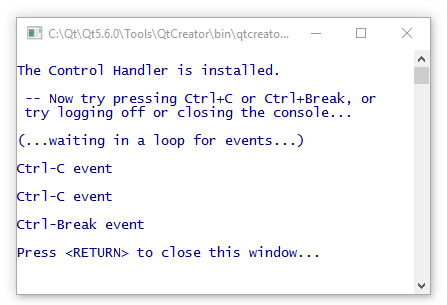
\includegraphics[scale=0.8]{task7}}
		\caption{Результат работы}
		\label{img:task7}
	\end{figure}
	Так как сигналы не являются средством IPC в Windows, а средством пользователя и системы с процессом, то можно предположить что собственные обработчики сигналов задуманы для корректного завершения программы, например, закрытия всех поток и корректное окончание записи файлов, для которых простой обрыв неприемлем. Так реализуем популярный в программах с графическим интерфейсом вопрос "Уверены ли вы, что хотите закрыть программу". Для этого изменим обработчик:
	\begin{lstlisting}[style=crs_cpp]
	printf( "Do you want to close this app?\nPress Ctrl-C one more time to close it...\n\n" );
	SetConsoleCtrlHandler((PHANDLER_ROUTINE)CtrlHandler, FALSE);
	return( TRUE ); //CTRL-CLOSE: confirm that the user wants to exit. \end{lstlisting}

	Результат выполнения программы при двухкратном нажатие Ctrl-C приведен на рисунке \ref{img:task7_1}.
	\begin{figure}[h!]
		\center{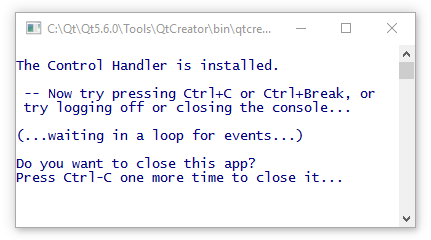
\includegraphics[scale=0.8]{task7_1}}
		\caption{Результат работы с собственным обработчиком}
		\label{img:task7_1}
	\end{figure}
	
	Программа при первом сигнале попадает в свой обработчик, где выводит инструкцию пользователю и устанавливает обработчик по умолчанию. При втором сигнале вызывается обработчик по умолчанию, а он приводит к завершению процесса.
	
\subsection{Разделяемая память}
	Потоки одного процесса могут разделять общую память этого процесса. У каждого процесса – свое изолированное адресное пространство. Кроме рассмотренных выше средств передачи информации между процессами или потоками разных процессов, одно из наиболее эффективных – использование общей памяти, доступ к которой обеспечивается со стороны каждого процесса. ОС Windows поддерживает такое средство, как именованная, совместно используемая память.
Приведем системные функции, которые позволяют запрограммировать такое взаимодействие.
	
	Первый участвующий в обмене информацией процесс создает объект "проекция файла" при помощи вызова функции CreateFileMapping(). Используя флажок \texttt{PAGE\_READWRITE}, задается доступ по чтению и записи в память через представление данных файла в адресном пространстве процесса. Процесс затем использует дескриптор объекта "проекция файла", возвращаемый функцией CreateFileMapping(), при вызове функции MapViewOfFile(). Эта функция создает представление файла в адресном пространстве процесса и возвращает указатель на представление данных файла для их дальнейшего использования.
	
	Другой процесс может получить доступ к тем же данным при помощи вызова функции OpenFileMapping() с тем же самым именем, что и первый процесс, а затем использовать функцию MapViewOfFile(), чтобы получить свой указатель на представление данных файла.
	
	Для записи данных в память используется функция CopyMemory(), первый аргумент которой – возвращаемый функцией MapViewOfFile() указатель, а следующие – характеризуют записываемые данные.
	
	Когда процессу больше не нужен доступ к объекту "проекция файла в память", он должен вызвать функцию CloseHandle() для дальнейшего освобождения ресурса. При условии, что все дескрипторы закрыты (не осталось процессов, использующих этот ресурс), система может освободить секцию файла подкачки, используемого объектом.
	
	\textbf{Задание} Создать программу, в которой первый процесс генерирует случайное число и записывает его в буфер, доступный второму процессу, откуда он его и считывает с последующим выводом.
	
	Исходный код первой:
	\lstinputlisting[style=crs_cpp]{shmem_writer.cpp}
	
	Исходный код второй программы:
	\lstinputlisting[style=crs_cpp]{shmem_reader.cpp}
	
	Результат выполнения программы приведен на рисунке \ref{img:task8}.
	\begin{figure}[h!]
		\center{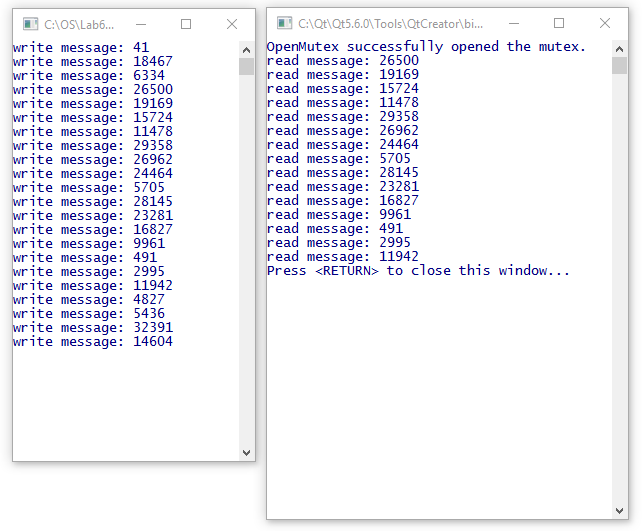
\includegraphics[scale=0.8]{task8}}
		\caption{Результат работы}
		\label{img:task8}
	\end{figure}
	
	Для организации синхронизации доступа к памяти в данном примере рассматривается использование мьютексов. В первом процессе создается именованный мьютекс, который "защищает" критические участки кода, в данном случае - запись в общую разделяемую память.
	
	Записываемая в буфер информация - это случайное число, которое генерируется функцией rand()перед каждой записью.
	
	Сообщения извлекаются из памяти правильно, следовательно, система разделения доступа к памяти работает корректно.
	
\subsection{Почтовые слоты}
	MailSlot – механизм синхронизации, иначе называемый «почтовый ящик». Каждый слот реализуется как псевдофайл в оперативной памяти и содержит некоторое количество записей («сообщений»), которые могут быть прочтены всеми компьютерами в сетевом домене. Общий размер данных не дможет превышать 64K. В отличие от дисковых файлов, файлы MailSlot временные. Когда все указатели на MailSlot закрываются, MailSlot и все данные, которые он содержит, удаляются. Для обмена посредством MailSlot создается клиент-серверное приложение. MailSlot сервер – является процессом, который создает и владеет MailSlot. При создании сервер получает указатель, используемый затем при чтении или записи данных им самим или другим процессом, получившим указатель на MailSlot. Создать слот можно только локально, а получать доступ (обращаться) и локально и удалённо.
	
	Для демонстрации работы с почтовыми слотами были написаны программы сервера и клиента.	Исходный сервера:
	\lstinputlisting[style=crs_cpp]{mailslot_server.cpp}
	
	Исходный код клиента:
	\lstinputlisting[style=crs_cpp]{mailslot_client.cpp}
	
	Результат локального выполнения программ приведен на рисунке \ref{img:task9}.
	\begin{figure}[h!]
		\center{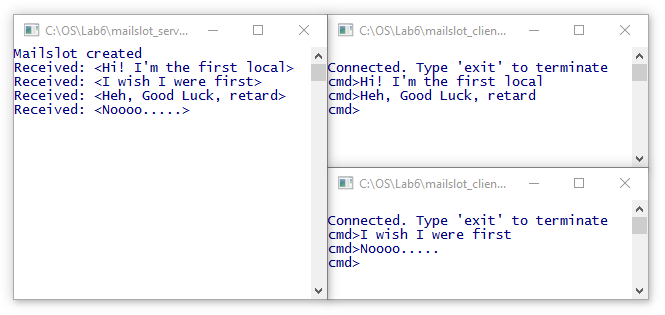
\includegraphics[scale=0.8]{task9}}
		\caption{Локальный запуск}
		\label{img:task9}
	\end{figure}
	
	Используя почтовые слоты можно передавать данные между компьютерами в локальной сети. Для этого клиенту укажем имя основной машины "WIN-IS-HARD".
	
	Результат сетевого выполнения программ приведен на рисунках \ref{img:task9_net_local} и \ref{img:task9_net_remote}.
	\begin{figure}[h!]
		\center{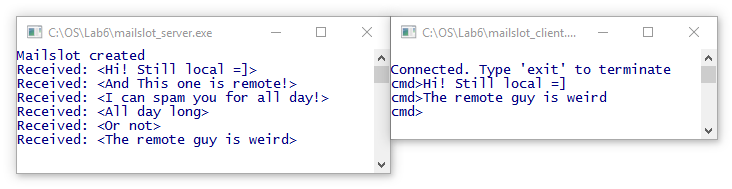
\includegraphics[scale=0.8]{task9_net}}
		\caption{Сетевой запуск на локальной машине}
		\label{img:task9_net_local}
	\end{figure}

	\begin{figure}[h!]
		\center{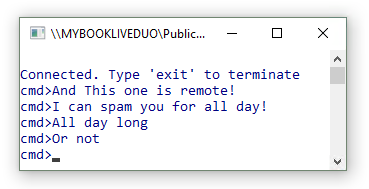
\includegraphics[scale=0.8]{task9_net_remote}}
		\caption{Сетевой запуск на дополнительной машине}
		\label{img:task9_net_remote}
	\end{figure}
	
	Для подтверждения работы по сети был записан соответствующий трафик. Он представлен на рисунке \ref{img:task9_wire}
	
	\begin{figure}[h!]
		\center{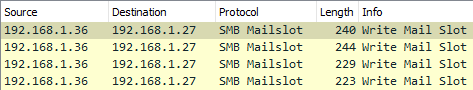
\includegraphics[scale=0.9]{task9_wire}}
		\caption{Запись трафика основной машиной}
		\label{img:task9_wire}
	\end{figure}
	
	Учитывая, что фильтрация была по протоколу, мы видим, что локальный трафик не выходит в сеть, а все попавшие в сеть пакеты соответствуют своему отправленному из дополнительной машины сообщению.\\
	
	При создании почтовых слотов с одинаковым именем на нескольких компьютерах домена возможна широковещательная рассылка сообщений клиентов. Один клиентский процесс может посылать сообщения сразу всем этим серверным процессам. Для этого заменим в клиенте имя компьютера на символ '*'. Запустим на каждой из машин по серверу и по широковещательному клиенту:
	
		Результат широковещательного выполнения программ приведен на рисунках \ref{img:task9_broad_local} и \ref{img:task9_broad_remote}.
	\begin{figure}[h!]
		\center{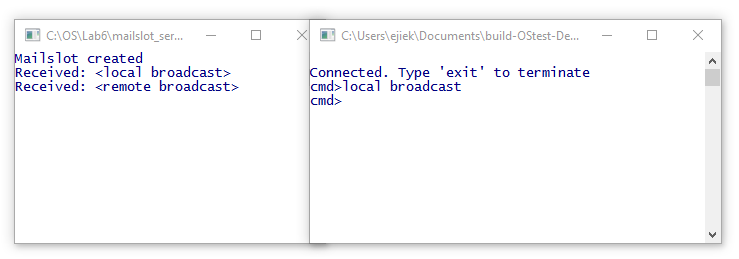
\includegraphics[scale=0.8]{task9_broad_local}}
		\caption{Широковещательный запуск на локальной машине}
		\label{img:task9_broad_local}
	\end{figure}

	\begin{figure}[h!]
		\center{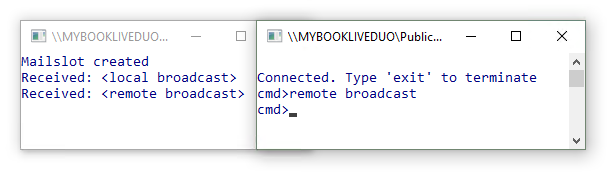
\includegraphics[scale=0.8]{task9_broad_remote}}
		\caption{Широковещательный запуск на дополнительной машине}
		\label{img:task9_broad_remote}
	\end{figure}
	
	Для подтверждения работы по сети был записан соответствующий трафик. Он представлен на рисунке \ref{img:task9_broad_wire}
	
	\begin{figure}[h!]
		\center{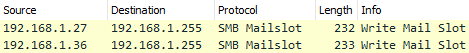
\includegraphics[scale=0.9]{task9_broad_wire}}
		\caption{Запись трафика основной машиной}
		\label{img:task9_broad_wire}
	\end{figure}

\section{Вывод}
	В ОС Windows реализовано несколько средств межпроцессного взаимодействия. Некоторые из них совпадают с IPC в UNIX: неименованные и именованные каналы, сокеты, разделяемая память. Некоторые уникальны, например, почтовые слоты.
	
	Неименованные каналы Windows обеспечивают однонаправленное (полудуплексное) посимвольное межпроцессное взаимодействие. Каждый канал имеет два дескриптора: дескриптор чтения и дескриптор записи. Дескрипторы каналов часто бывают наследуемыми. Чтобы канал можно было использовать для IPC, должен существовать еще один процесс, и для этого процесса требуется один из дескрипторов канала. 
Анонимные каналы обеспечивают только однонаправленное взаимодействие. Для двухстороннего взаимодействия необходимы два канала. 

	Именованные каналы обеспечивают межпроцессное взаимодействие между сервером и одним или несколькими клиентами. Они предоставляют больше функциональных возможностей, чем анонимные каналы, которые обеспечивают межпроцессное взаимодействие на локальном компьютере. Именованные каналы поддерживают дуплексную связь по сети, несколько экземпляров сервера, взаимодействие, основанное на сообщениях и олицетворение клиента, что позволяет подключаемым процессам использовать собственные наборы разрешений на удаленных серверах. Использовать именованные каналы для связи по сети возможно только для компьютеров с ОС Windows, подключенных к одной домашней группе. Поэтому, именованные каналы редко используются для клиент-серверных приложений.
	
	Возможность взаимодействия с другими системами обеспечивается в Windows поддержкой сокетов. Сокет – это оконечная точка соединения, которая идентифицируется 4 значениями: IP адрес отправителя, порт отправителя, IP адрес получателя, порт получателя. 
	
	Механизм сигналов как IPC отсутствует в ОС Windows. Процессы не могут отправлять сигналы другим процессам для обмена информацией. Присутствует 2 сигнала которые пользователь может отправлять приложению с клавиатуры: Ctrl+C и Ctrl+Break. Так же система может посылать приложению сигналы когда пользователь закрывает консоль, выходит из системы или когда система завершается.
	
	ОС Windows поддерживает такое средство, как именованная, совместно используемая память. Разделяемая память позволяет обмениваться информацией между двумя процессами.
	
	MailSlot – механизм синхронизации, иначе называемый «почтовый ящик». Каждый слот реализуется как псевдофайл в оперативной памяти и содержит некоторое количество записей («сообщений»), которые могут быть прочтены всеми компьютерами в сетевом домене. Используя почтовые слоты можно передавать данные между компьютерами в локальной сети. При создании почтовых слотов с одинаковым именем на нескольких компьютерах домена возможна широковещательная рассылка сообщений клиентов. Один клиентский процесс может посылать сообщения сразу всем этим серверным процессам.

\section{Список литературы}
\begin{itemize}
\item Душутина Е.В.  Межпроцессные взаимодействия в операционных системах – СПб, 2014 г, 136 с.
\item Душутина Е.В.  Практические вопросы оазработки системных приложений – СПб, 2015 г, 165 с.
\item Таненбаум Э., Бос Х. Современные операционные системы. 4-е изд. – СПб.: Питер, 2015 – 1120 с.
\end{itemize}
	

\end{document}

